
學習線程安全的數據結構之前,必須知道需要哪些數據結構。如果這是一個簡單的問題——多個線程可以同時使用的數據結構——那麼你還太天真了。開始設計併發程序中使用的新數據結構或算法時,就知道這個問題有多麼重要了,以至於怎麼強調都不為過。這句話應該讓你感到警惕,並停下來思考。實際情況是,線程安全的數據結構沒有一個明確定義適合每種需求和應用程序。

\subsubsubsection{7.2.1\hspace{0.2cm}線程安全的最佳方式}

可以從一些簡單的,但在實踐中容易遺忘的方式開始。高性能設計的一個原則是,\textit{不做總是比做要快}。當前,這個原則可以縮小為,對於數據結構是否需要線程安全?確保線程安全,意味著需要由計算機完成一些工作,我們真的需要嗎?是否可以對計算進行調度,使每個線程都有自己的數據集進行操作?

在前一章中使用的線程安全計數器。如果所有線程始終看到計數器的當前值,這就是正確的解決方案。但當所需要的只是計算在多個線程上發生的事件,例如:分配給多個線程的一組大數據中搜索某些內容。線程在執行搜索時不需要知道計數的當前值。當然,需要知道計數的最新值來增加它,這是正確的,只有在所有線程上增加單個共享計數時才會出問題,就像這樣:

\hspace*{\fill} \\ %插入空行
\noindent
\textbf{01a\_shared\_count.C}
\begin{lstlisting}[style=styleCXX]
std::atomic<unsigned long> count;
…
for ( … counting loop … ) { // On each thread
	… search …
	if (… found …)
	count.fetch_add(1, std::memory_order_relaxed));
}
\end{lstlisting}

計數的性能非常差,可以看到在基準測試中只做計數(不搜索):

%\hspace*{\fill} \\ %插入空行
\begin{center}
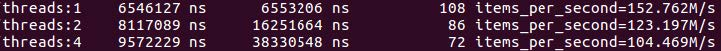
\includegraphics[width=0.9\textwidth]{content/2/chapter7/images/1.jpg}\\
圖7.1 - 如果計數是共享的,對多個線程的計數不會修改
\end{center}

計數的改變實際上是負的,在兩個線程上獲得相同的計數要比在一個線程上花費更長的時間(儘管已經盡最大努力使用無等待的計數,同時使用最快的內存序)。當然,如果搜索比計數要長,那麼計數的性能就無關緊要了(但搜索代碼本身也可以在全局數據上做一些事,或者在每個線程的副本上做一些事,所以這是一個有指導意義的例子)。

假設只關心計算結束時的計數值,一個更好的解決方案是,在每個線程上保持本地計數,並且只增加共享計數一次:

\hspace*{\fill} \\ %插入空行
\noindent
\textbf{01b\_per\_thread\_count.C}
\begin{lstlisting}[style=styleCXX]
unsigned long count;
std::mutex M; // Guards count
…
// On each thread
unsigned long local_count = 0;
for ( … counting loop … ) {
	… search …
	if (… found …) ++local_count;
}
std::lock_guard<std::mutex> L(M);
count += local_count;
\end{lstlisting}

為了強調共享計數增量的不重要性,將使用互斥鎖對其進行保護。通常,鎖是更安全的選擇,因為它更容易理解(因此,更難製造Bug),儘管在計數的情況下,原子整數會讓代碼更簡單。

如果每個線程在到達結束之前多次增加本地計數,並且必須對共享計數進行增加的操作,那麼這種變化幾乎完美:

%\hspace*{\fill} \\ %插入空行
\begin{center}
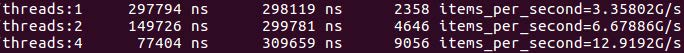
\includegraphics[width=0.9\textwidth]{content/2/chapter7/images/2.jpg}\\
圖7.2 - 在多個線程上完美地計數
\end{center}

最好的線程安全是,不需要多個線程訪問共享數據。通常,這種安排會以一些開銷為代價,例如:每個線程維護一個容器或內存分配器,其大小會不斷地改變。在程序結束之前不將內存釋放給主分配程序,就可以避免鎖定。代價是一個線程上未使用的內存不能提供給其他線程使用,因此總的內存使用將是所有線程峰值的總和(即使這些峰值使用時刻發生在不同的時間)。這是否可以接受取決於問題的細節和實現,這是每個開發者都必須考慮的問題。

當涉及到線程安全時,這個方案選擇了逃避。從某種角度來看,確實如此,但在實際中經常出現這樣的情況。在不需要共享數據結構的地方使用共享數據結構,並且性能提高非常明顯,因此需要強調這一點。現在是時候來看看真正的線程安全了,其中數據結構必須在線程之間共享。

\subsubsubsection{7.2.2\hspace{0.2cm}真正的線程安全}

假設確實需要同時從多個線程訪問特定的數據結構,現在就必須討論線程安全了。但現在還是沒足夠的信息來確定線程安全意味著什麼。前一章中討論了強線程和弱線程安全保證。本章中,這樣的分區已經不夠了,所以這裡不討論一般的線程安全,而是應該描述數據結構提供併發訪問的保證。

弱(但通常很容易提供)保證只要數據結構保持不變,多個線程就可以對相同的數據結構進行讀取操作。顯然,任意數量線程可以隨時執行任何操作,並且數據結構保持在良好定義的狀態,這種保證通常既昂貴又不必要。程序可能需要數據結構支持的某些(但不是所有)操作提供這樣的保證。還有其他的簡化版本,比如:限制訪問數據結構的線程數量。

想要提供儘可能少的保證來保證程序是正確的,線程安全特性通常非常昂貴,甚至不使用時也會產生開銷。

考慮到這一點,就可以開始研究具體的數據結構了,並看看如何提供不同級別的線程安全。

































